\documentclass[a4paper]{article}
\usepackage[T1]{fontenc}
\usepackage[utf8]{inputenc}
\usepackage[french]{babel}
\usepackage{graphicx}
\usepackage{wrapfig}
\usepackage{caption}
\usepackage{geometry}
\usepackage{amsmath,amsfonts,amssymb}
\usepackage{changepage}
\usepackage{eurosym}
\usepackage{dsfont}
\usepackage{stmaryrd}
\usepackage{algorithm}
\usepackage{algorithmicx}
\usepackage{algpseudocode}
\usepackage{turnstile}
\usepackage{mathrsfs}
\usepackage{enumitem}
\usepackage{tikz}
\usepackage{amsthm}
\usepackage[super]{nth}
\usepackage[toc,page]{appendix}
\usepackage{listings}
\usepackage{listings}
\usepackage{mathtools}
\usepackage{csquotes}
\usepackage{multicol}
\usepackage{fancyvrb}
\usepackage{makecell}
\usepackage[toc,page]{appendix}
\usepackage{mdframed}
\usepackage{setspace}
\usepackage{tcolorbox}
\usepackage[sc,osf]{mathpazo}
\usepackage{array}
\usepackage{subcaption}

\lstset{
  basicstyle=\ttfamily,
  mathescape
}


\usepackage[unicode=true, bookmarks=false, breaklinks=true, pdfborder={0 0 1},colorlinks=true]{hyperref}
\hypersetup{linkcolor=blue,citecolor=blue,filecolor=blue,urlcolor=blue}

\usetikzlibrary{automata, positioning, calc, shapes, snakes}

\geometry{hmargin=2.4cm, vmargin=2.5cm}

\theoremstyle{plain}
\newtheorem{theorem}{Théorème}
\newtheorem{lemma}{Lemme}
\newtheorem{corollary}{Corollaire}
\newtheorem{example}{Exemple}
\newtheorem{conjecture}{Conjecture}

\newenvironment{point}[1]%
{\subsection*{#1}}%
{}

\usepackage{fancyhdr}
\pagestyle{fancy}
\fancyhead[l]{\emph{}}
\fancyhead[r]{\emph{}}

\renewcommand{\headrulewidth}{0pt}
\usepackage{sectsty}
\sectionfont{\rmfamily\mdseries\Large}
\subsectionfont{\rmfamily\mdseries\itshape\large}

\newcommand{\HRule}{\rule{\linewidth}{0.5mm}}

\begin{document}
{\centering \noindent \huge Projet MADI -- Processus de décision Markovien et apprentissage par renforcement.}
\vspace{0.5cm}\\
{\Large Defiolles Julien et Rey Simon}

\vspace{0.8cm}

Le but de ce projet est de développer une application permettant de résoudre des labyrinthes non déterministes. Il s'appuie pour cela sur la résolution des processus de décision Markovien ainsi que l'apprentissage par renforcement.

Le projet est développé en Python et utilise le logiciel sous licence Gurobi pour le résolution des programmes linéaires, pour l'affichage graphique la librairie pygame est utilisée.

\paragraph{Notations.} On considère dans la suite un donjon carré donné. On note $n$ la taille du donjon définit le nombre de cases dans une ligne (ou une colonne) du donjon, le donjon a donc $n \times n$ cases. La case départ est la case à la position $(n - 1, n - 1)$ et le trésor est en position $(0, 0)$. On note $\mathcal{C}$ l'ensemble des positions pour lesquelles il n'y a pas de mur. Pour une position $p \in \llbracket 0, n- 1\rrbracket \times \llbracket 0, n- 1\rrbracket$, on note $adj(p)$ les positions adjacentes qui ne sont pas des murs.

\section{Gestion des donjons}

Pour représenter les donjons nous avons développé une classe \texttt{Dungeon} qui stocke un donjon comme une matrice de case, chaque case étant définit par son type (Clé, Piège, Trésor, Portail...). 

Cette classe nous permet de créer un donjon à partir d'un fichier définissant un donjon selon le standard suivant : la première ligne donne la dimension du donjon les coordonnées étant séparées par un espace, les autres lignes définissent les cases du donjon, ligne par ligne sans séparateur. Les caractères utilisés pour chaque case sont donnés en Table \ref{tab:case}.
\begin{table}
	\centering
	\begin{tabular}{>{\begin{center}}m{1.7cm}<{\end{center}}|>{\begin{center}}m{1.5cm}<{\end{center}}|>{\begin{center}}m{1.7cm}<{\end{center}}|m{40pt}||>{\begin{center}}m{1.7cm}<{\end{center}}|>{\begin{center}}m{1.5cm}<{\end{center}}|>{\begin{center}}m{1.7cm}<{\end{center}}|m{40pt}}
		\textbf{Case} & \textbf{Caractère associé} & \textbf{Probabilité de création} & \begin{center} \textbf{Image utilisée}\end{center} & \textbf{Case} & \textbf{Caractère associé} & \textbf{Probabilité de création} & \begin{center} \textbf{Image utilisée}\end{center}\\
		\hline
		Mur & w & 0.2 & 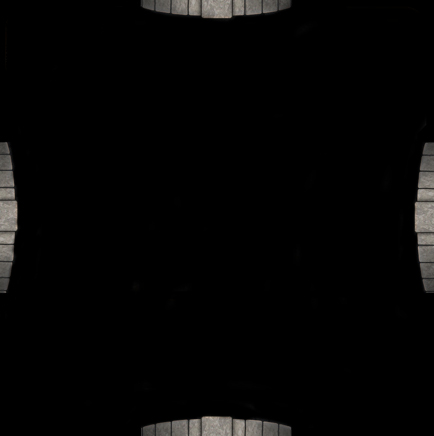
\includegraphics[height=40pt]{../Code/resources/tileWall.jpg} & 
		Vide & \textvisiblespace & 0.4 & 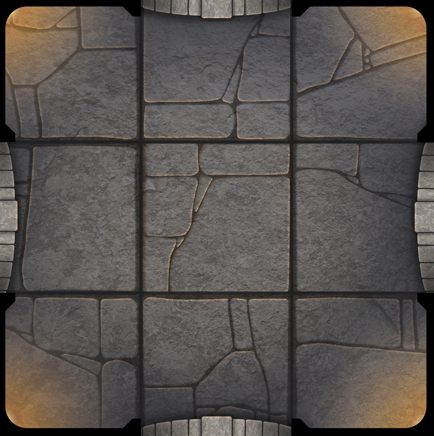
\includegraphics[height=40pt]{../Code/resources/tileEmpty.jpg}\\
		Ennemie & e & 0.1 & 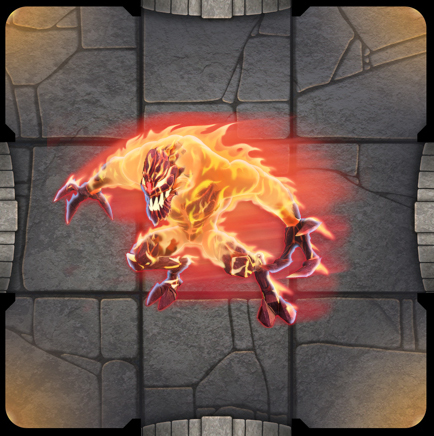
\includegraphics[height=40pt]{../Code/resources/tileEnemy.jpg}&
		Piège & r & 0.1 & 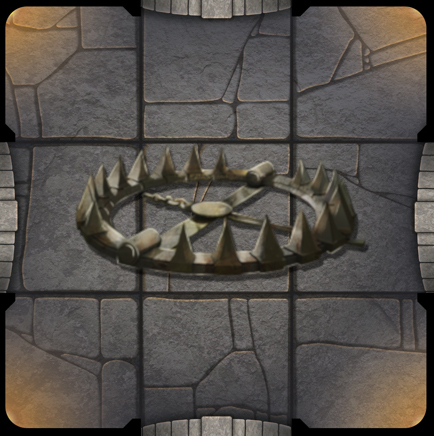
\includegraphics[height=40pt]{../Code/resources/tileTrap.jpg} \\
		Fissure & c & 0.05 & 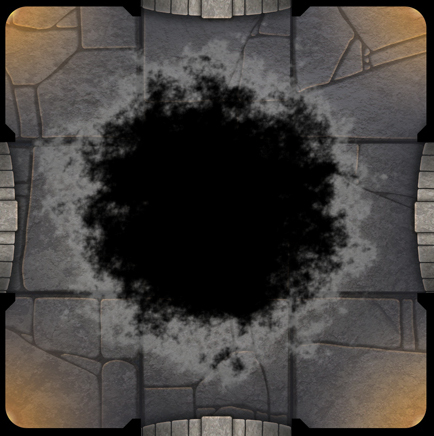
\includegraphics[height=40pt]{../Code/resources/tileCrack.jpg} &
		Portail & p & 0.05 & 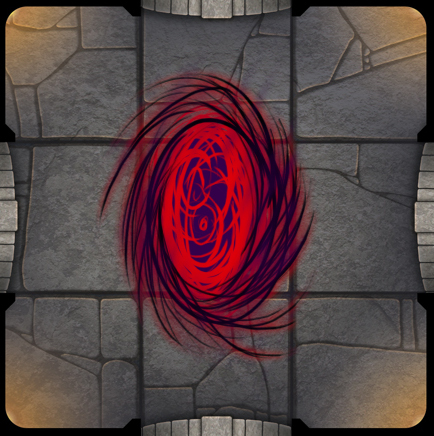
\includegraphics[height=40pt]{../Code/resources/tilePortal.jpg} \\
		Plateforme & \_ & 0.1 & 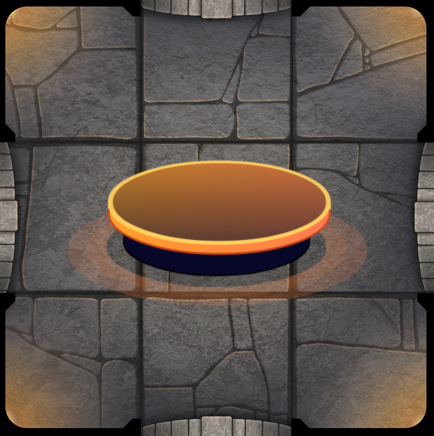
\includegraphics[height=40pt]{../Code/resources/tilePlatform.jpg} &
		Départ & o &  & 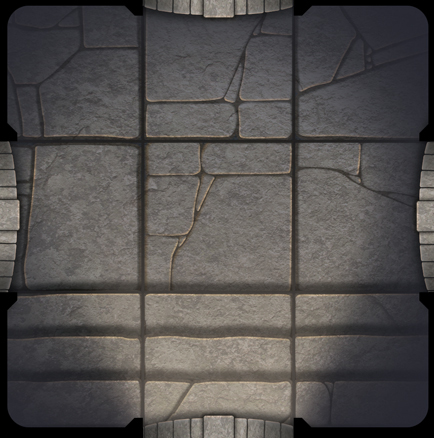
\includegraphics[height=40pt]{../Code/resources/tileStart.jpg}\\
		Trésor & t &  & 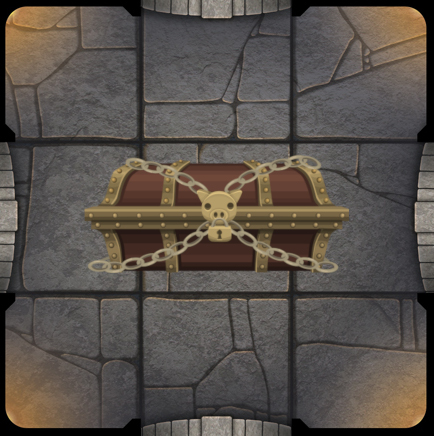
\includegraphics[height=40pt]{../Code/resources/tileTreasure.jpg} &
		Épée & s &  & 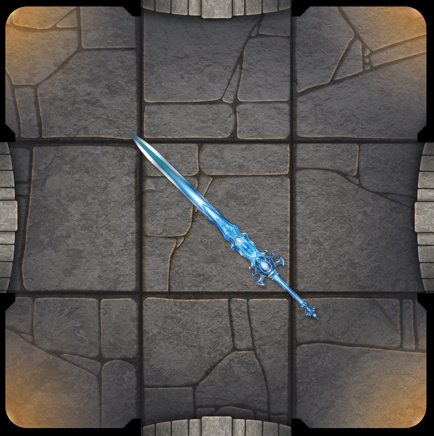
\includegraphics[height=40pt]{../Code/resources/tileSword.jpg}\\
		Clé & k & & 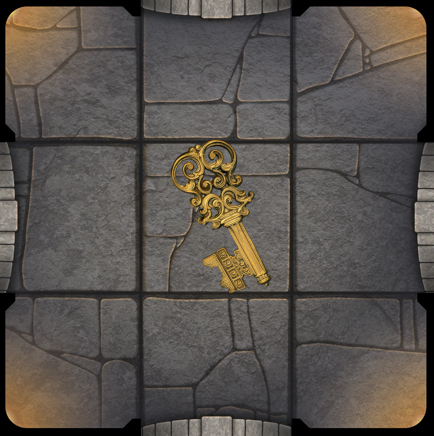
\includegraphics[height=40pt]{../Code/resources/tileKey.jpg} & 
		Héro & & & 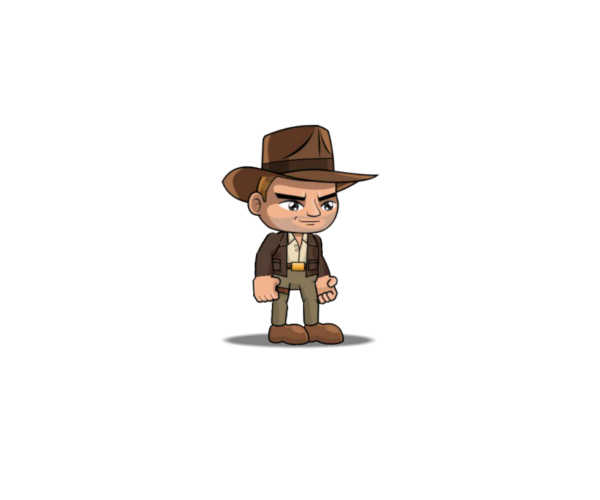
\includegraphics[height=40pt]{../Code/resources/hero.png}
	\end{tabular}
	\caption{Informations sur les cases des donjons}
	\label{tab:case}
\end{table}

Ainsi le donjon donné dans l'énoncé s'écrit :
\begin{center}
\begin{BVerbatim}
8 8
te  rwck
wrww_c_r
_ e   _r
pw _p_r 
swwew ww
_r  r_cp
wwew w  
e      o
\end{BVerbatim}
\end{center}

La classe permet aussi d'écrire un donjon dans un fichier, ce qui permet de les sauvegarder.

Les donjons peuvent aussi être générer aléatoirement, dans ce cas les cases obligatoires (Départ, Trésor, Clé et Épée) sont positionnées dès le départ, les autres cases sont remplies en suivant les probabilités données dans la table précédente.

L'amélioration que nous avons décidé de mettre en \oe uvre est de prendre en compte des points de vie pour le joueur. Ainsi à la création d'un joueur un paramètre défini ses points de vie initiaux. Nous avons donc changé les effets de certaines cases, les ennemies et les pièges retirent donc des points de vie plutôt que de tuer le joueur (voir la fonction de transition du PDM en Table \ref{tab:transition} pour plus de précisions).

\section{Déroulement d'une partie}

La classe \texttt{State} définie les états d'une partie (position, possessions et vie du joueur). C'est aussi dans cette classe qu'est implémentée la fonction d'évaluation des états pour le PDM.

Nous avons aussi créé une classe \texttt{Player} qui permet de représenter le joueur. On y retrouve sa position, les objets qu'il possède ainsi que ses points de vie. Cette classe peut sembler ne pas apporter d'informations supplémentaires que la classe \texttt{State}, cependant cela permet d'avoir une organisation du projet plus cohérente du point de vue sémantique et permet de bien séparer les méthodes spécifiques aux deux.

La classe \texttt{Graphics} gère l'affichage de la partie grâce à la librairie \texttt{pygame}. Elle permet d'afficher un dongeon, les déplacements du joueur, des messages ainsi que la stratégie calculée par les PDM. \\

Le déroulement d'une partie est le suivant :
\begin{itemize}
	\item Le mouvement du joueur est récupéré (dans la politique optimale du PDM ou par les entrées de l'utilisateur)
	\item La méthode \texttt{move} de la classe \texttt{Player} est appelée avec ce mouvement. Cette dernière réalise les actions suivantes :
	\begin{itemize}
		\item Elle applique le mouvement du joueur en le déplaçant sur la case suivante
		\item Elle applique toutes les réactions de la nouvelle case (attaque d'ennemies, téléportation par le portail...)
		\item Si de nouvelles réactions doivent être appliquée à cause des réactions précédentes (téléportation d'un portail qui déclenche une attaque d'ennemie), elles sont appliquées jusqu'à épuisement des réactions.
	\end{itemize}
	\item Si à l'issue du déplacement la partie se termine (victoire ou défaite) un message est affiché et le programme se termine. Sinon la même boucle continue.
\end{itemize}

\section{Modélisation par les processus décisionnels Markoviens}

\begin{table}
	\centering
	\begin{tabular}{c|c|c}
		\textbf{Type de case} & \textbf{Nouvel état} & \textbf{Probabilité}\\
		\hline
		Départ & $\langle t, s, k, pos, life \rangle$ & 1 \\
		\hline
		Vide & $\langle t, s, k, pos, life \rangle$ & 1\\
		\hline
		Clé & $\langle t, s, True, pos, life \rangle$ & 1 \\
		\hline
		Épée & $\langle t, True, k, pos, life \rangle$ & 1 \\
		\hline
		Trésor et $k = True$ & $\langle True, s, k, pos, life \rangle$ & 1 \\
		\hline
		Trésor et $k = False$ & $\langle t, s, k, pos, life \rangle$ & 1 \\
		\hline
		Fissure & $\langle t, s, k, pos, 0 \rangle$ & 1 \\
		\hline
		Ennemie et $s = True$ & $\langle t, s, k, pos, life \rangle$ & 1 \\
		\hline
		Ennemie et $s = False$ & $\langle t, s, k, pos, life - 1 \rangle$ & 0.3 \\
		& $\langle t, s, k, pos, life \rangle$ & 0.7 \\
		\hline
		& $\langle t, s, k, pos, life \rangle$ & 0.6 \\
		Piège & $\langle t, s, k, pos, life - 1 \rangle$ & 0.1\\
		& $\langle t, s, k, (n - 1, n - 1), life \rangle$ & 0.3 \\
		\hline
		Plateforme & $\forall pos' \in adj(pos), \langle t, s, k, pos', life \rangle$ & $1 / |adj(pos)|$ \\
		\hline
		Portail & $\forall pos' \in \mathcal{C}\backslash\{pos\}, \langle t, s, k, pos', life \rangle$ & $1 / |\mathcal{C}\backslash\{pos\}|$
	\end{tabular}
	\caption{Fonction de transition du PDM}
	\label{tab:transition}
\end{table}

Un Processus Décisionnel Markovien (PMD) est défini par un tuple $\langle S, A, T, R \rangle$ où $S$ est un ensemble d'état, $A$ un ensemble fini d'actions, $T : S \times A \rightarrow L(S)$ une fonction de transition et $R : S\times A \rightarrow \mathbb{R}$ une fonction de récompense immédiate. Pour modéliser le jeu comme un PMD il nous faut donc définir l'ensemble de ces éléments. Nous avons choisi la représentation suivante :
\begin{itemize}
	\item Un état est un tuple $\langle t, s, k, pos, life \rangle$ où $t, k$ et $s$ sont des variables binaires représentant le fait que le joueur possède respectivement le trésor, l'épée ou la clé, $pos \in \llbracket 0, n- 1\rrbracket \times \llbracket 0, n- 1\rrbracket$ représente la position du joueur et $life \in \mathbb{N}$ son nombre de points de vie.
	
	L'ensemble $S$ est alors défini comme l'ensemble des états possibles, soit l'ensemble des couples $\langle t, s, k, pos, life \rangle$ possible tels que la case à la position $pos$ ne soit pas un mur.
	
	\item L'ensemble $A$ des actions correspond aux mouvement du joueur, on a donc $A = \{\rightarrow, \downarrow, \leftarrow, \uparrow\}$.
	
	Pour un état donné toutes les actions ne sont pas nécessairement disponibles, ainsi l'ensemble $A(st)$ des actions disponible pour un état $st = \langle t, s, k, pos, life \rangle$ dépend de la case à la position $pos$ :
	\begin{itemize}
		\item Si c'est une fissure (C), un portail (P), une plateforme (--) ou si le joueur est mort ($life = 0$), alors aucune action n'est possible, $T(st) = 0$
		\item Sinon $T(st) \subseteq \{\rightarrow, \downarrow, \leftarrow, \uparrow\}$ de telle sorte que l'action ne mène pas contre un mur (on considère que le donjon est entouré de mur).
	\end{itemize}

	\item La fonction de transition correspond à celle donnée dans l'énoncé. En partant d'un état $\langle t, s, k, pos_0, life \rangle$ et avec une action qui mène à une position $pos$, la fonction de transition est présentée en Table \ref{tab:transition}.

	\item La fonction d'évaluation des états est très simples tous les états donnent une récompense de $-1$ excepté l'état $\langle True, s, k, (n - 1, n - 1), life \rangle$ qui procure une récompense de $1 000 000$ et les états $\langle s, k, t, pos, 0\rangle$ qui procurent une récompense de $-1000$.
	
	Ainsi chaque pas est récompensé négativement pour pousser la résolution à choisir des chemins courts, mais c'est seulement en rapportant le trésor que le joueur peut marquer un score positif.
\end{itemize}

\section{Résolution du PDM}

Pour résoudre le PDM décrit ci-dessus nous avons implémenté l'algorithme d'itération de la valeur ainsi que la résolution par la programmation linéaire. 

Pour cela nous avons écrit une classe \texttt{BellmanEquation} dont une instance est créé pour chaque n\oe ud du PDM. Cette classe est centrale dans la résolution du PDM, la méthode \texttt{next\_value} retourne la nouvelle valeur d'un n\oe ud étant donné la valeur courante et la méthode \texttt{get\_contraints} retourne les contraintes du programme linéaire qui concerne le n\oe ud.

L'algorithme d'itération de la valeur procède de manière habituelle. En commençant avec une valuation arbitraire, il itère la méthode \texttt{next\_value} pour actualiser la valeur des n\oe uds. L'algorithme s'arrête dès lors que la précision est suffisante, c'est-à-dire dès lors que la différence entre la valuation courante et la valuation précédente est inférieure à 1.

La résolution par la programmation linéaire est classique, la méthode \texttt{get\_constraints} permet de générer toutes les contraintes du programme linéaire qui est ensuite résolu par Gurobi. \\
\begin{figure}
	\centering
	\begin{subfigure}[b]{0.48\textwidth}
		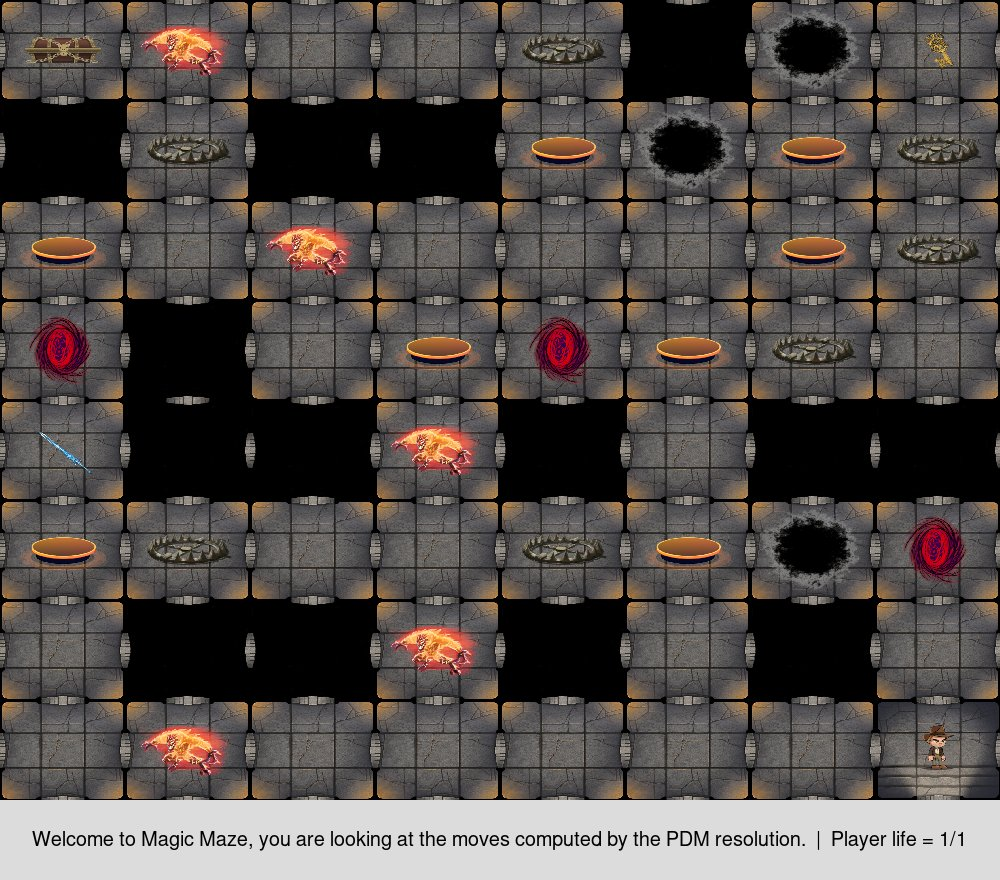
\includegraphics[width=\textwidth]{dungeonSujet.jpeg}
		\caption{Donjon}
	\end{subfigure}
	\begin{subfigure}[b]{0.48\textwidth}
		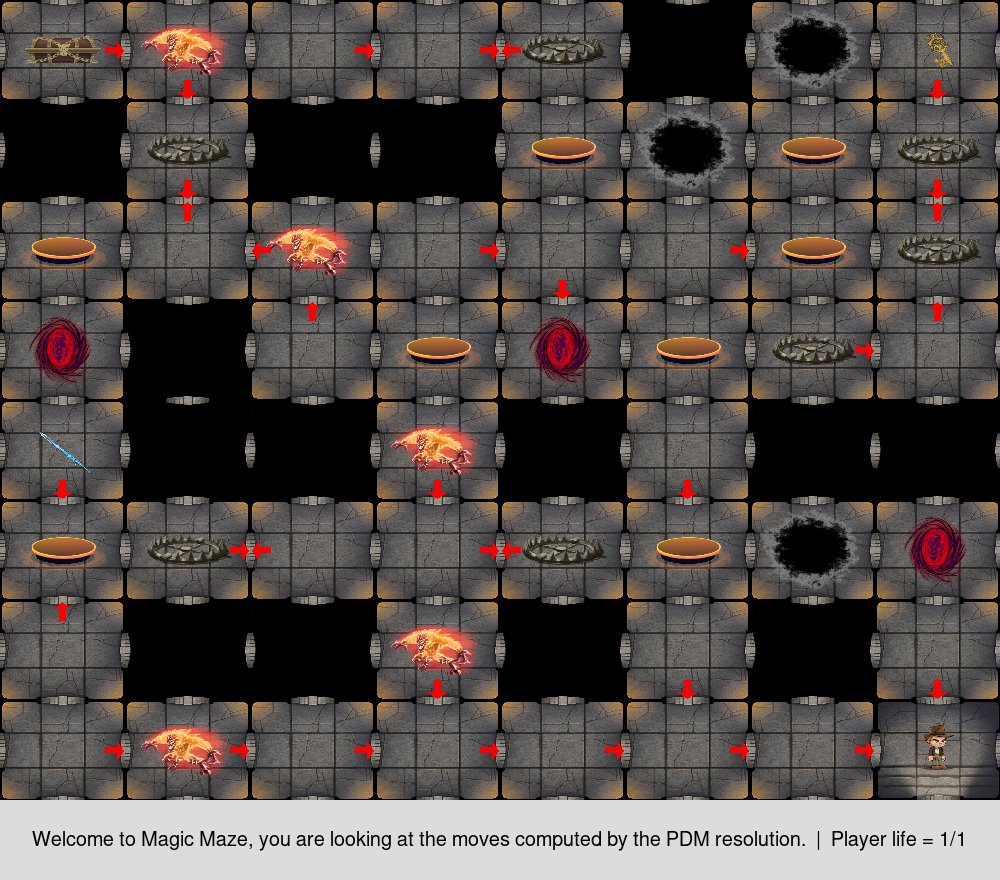
\includegraphics[width=\textwidth]{dungeonSujet_solTres.jpeg}
		\caption{Politique optimale pour renter avec le trésor}
	\end{subfigure}
	\begin{subfigure}[b]{0.48\textwidth}
		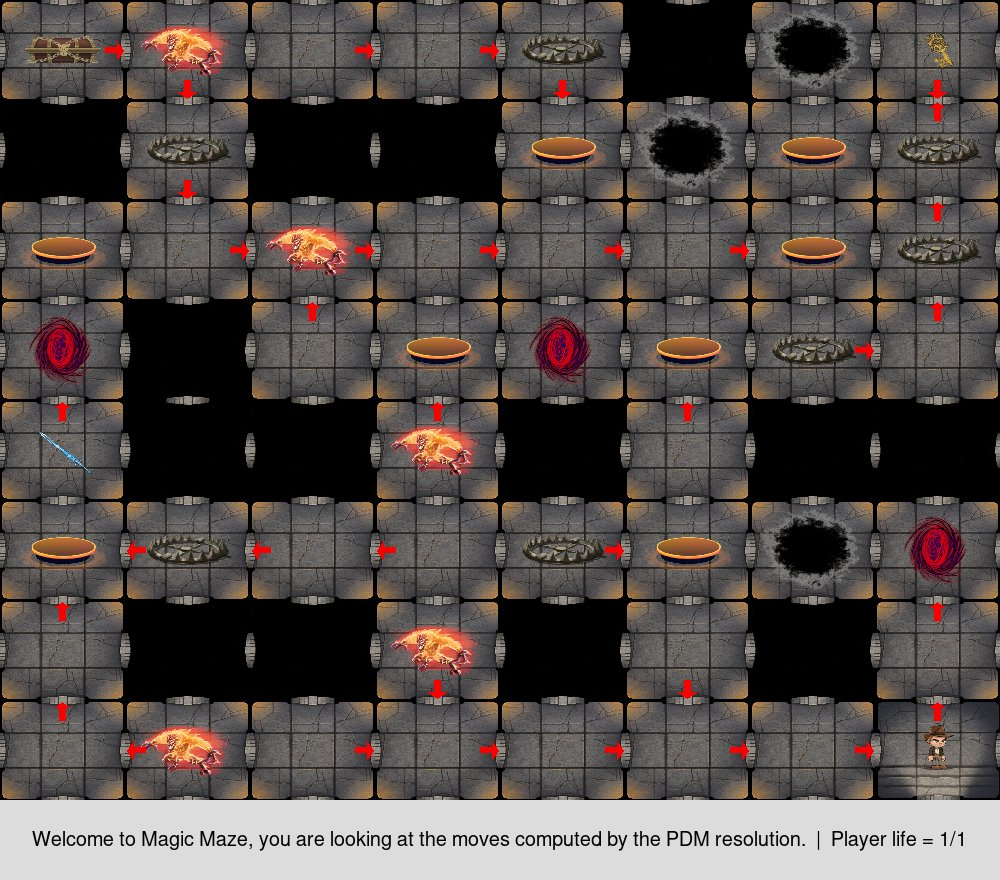
\includegraphics[width=\textwidth]{dungeonSujet_sol.jpeg}
		\caption{Politique optimale pour récupérer la clé}
		\label{fig:dclé}
	\end{subfigure}
	\begin{subfigure}[b]{0.48\textwidth}
		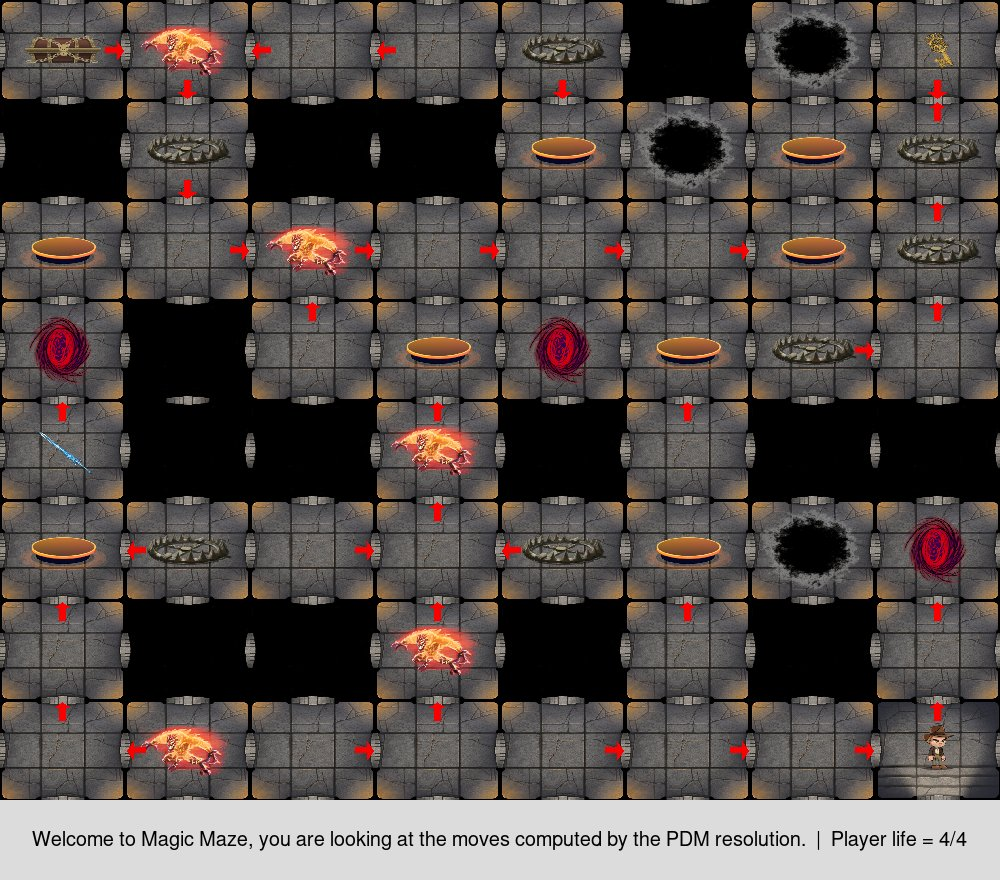
\includegraphics[width=\textwidth]{dungeonSujet_sol_life4.jpeg}
		\caption{Politique optimale pour la clé avec 4 points de vie}
		\label{fig:dclé4}
	\end{subfigure}
	\begin{subfigure}[b]{0.48\textwidth}
		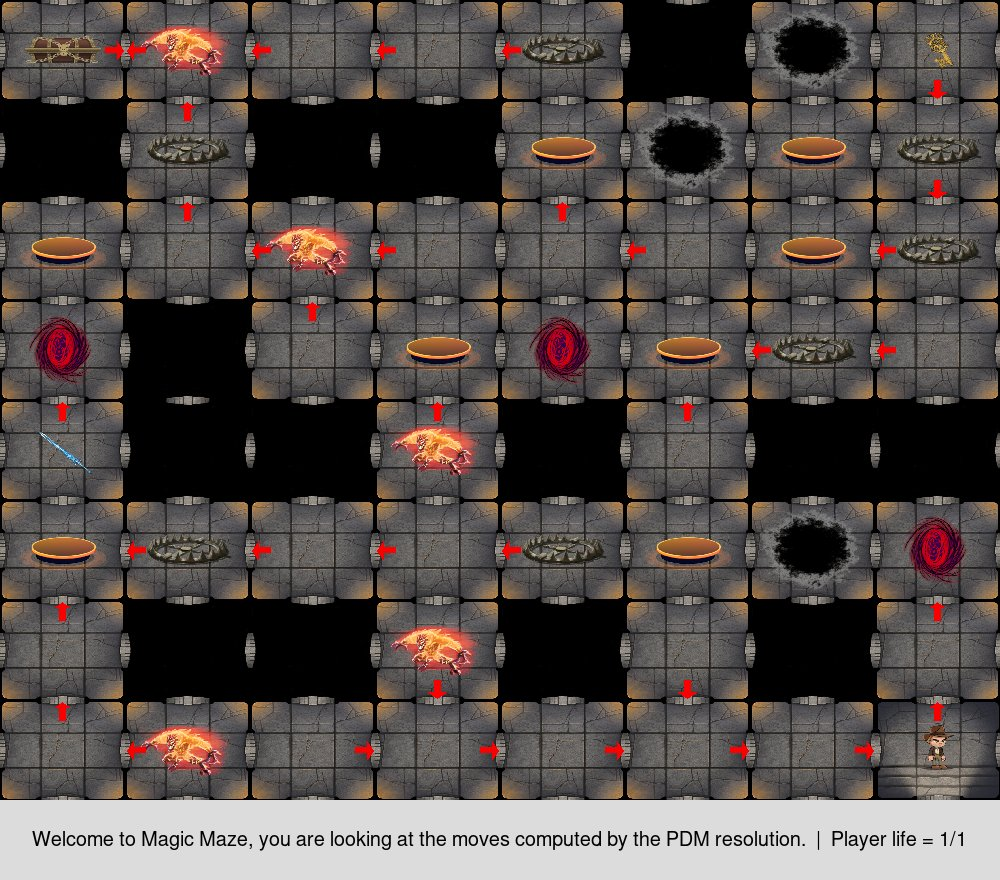
\includegraphics[width=\textwidth]{dungeonSujet_solKey.jpeg}
		\caption{Politique optimale pour aller chercher le trésor}
	\end{subfigure}
	\begin{subfigure}[b]{0.48\textwidth}
		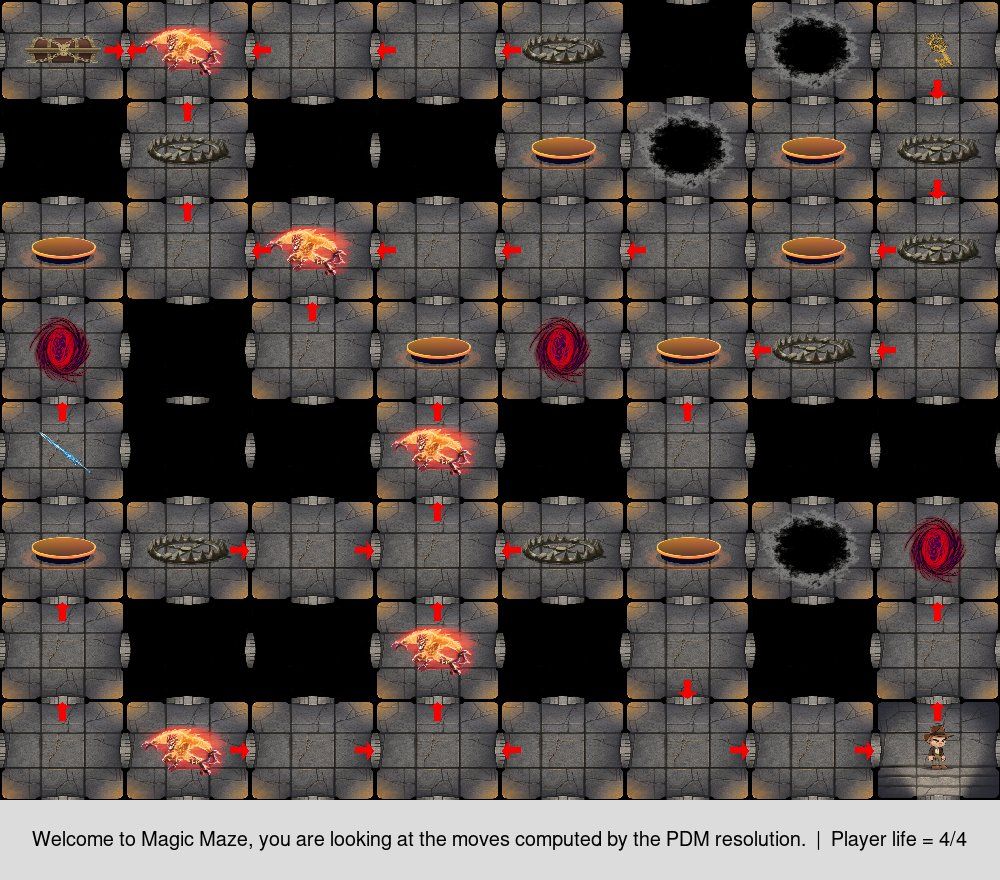
\includegraphics[width=\textwidth]{dungeonSujet_solKey_life4.jpeg}
		\caption{Politique optimale pour le trésor avec 4 points de vie}
	\end{subfigure}
	\caption{Politiques optimales pour le donjon de l'énoncé}
	\label{fig:donjonSujet}
\end{figure}


Un exemple de résolution est donné en Figure \ref{fig:donjonSujet} pour le donjon donné dans le sujet. Cinq politiques sont représentées : la politique initiale, celle lorsque le joueur possède la clé et celle lorsque le joueur possède le trésor et deux des politiques précédentes avec 4 points de vie. Ce n'est pas les seules politiques représentables, il faudrait aussi prendre en compte l'épée et tous les niveaux de points de vie. Il est intéressant d'observer les différences de politique lorsque le joueur a 4 points de vie. On observe alors que le joueur préfère combattre plusieurs ennemies (perte de points de vie) que de prendre le risque de tomber dans une fissure (mort assurée). Cela s'observe notamment sur les cases en haut à gauche entre les figures \ref{fig:dclé} et \ref{fig:dclé4}.

D'autres exemples de résolution avec des donjons de taille différente peuvent être trouvés dans le dossier Images de l'archive.

En termes de résolution il est intéressant de mentionner le fait que le joueur utilise très fortement les portails. En effet ces derniers permettant avec une probabilité assez importante de gagner du temps (et du de recevoir moins de récompenses de $-1$), notamment lorsque le joueur est loin de la case visée.

\section{Évaluation expérimental de la résolution du PDM}

Pour évaluer expérimentalement les performances de nos algorithmes, nous avons mesurer à la fois les temps de résolution et le nombre d'essai nécessaire pour gagner le donjon.

La procédure de test est la suivante :
\begin{itemize}
	\item Pour toute les tailles de donjon de 2 à 15, 10 instances sont générées
	\item Pour chaque instance, le temps de résolution et le nombre d'essai nécessaire pour gagner sont mesurer dix fois pour en prendre la moyenne
	\item Les graphiques sont ensuite tracés représentant les mesures selon la taille du donjon (moyenne sur les 10 instances d'une taille donnée et sur les 1O essais de chaque instance).
\end{itemize}

Les graphiques obtenus sont présentés en Figure \ref{fig:comparaisonAlgo} et \ref{fig:numIte}. 

La Figure \ref{fig:solveTime} indique clairement que la résolution par la programmation linéaire en utilisant Gurobi est supérieure pour résoudre le PDM. En effet sur les donjons de taille importante le temps de résolution est bien inférieur en utilisant Gurobi allant jusqu'à un facteur $1/15$ pour des donjons de taille 15. D'autres expérimentations ont permis de constater que Gurobi permet de résoudre rapidement des dunjons de taille 30, soit 900 cases.
\begin{figure}
	\centering
	\begin{subfigure}[b]{0.48\textwidth}
		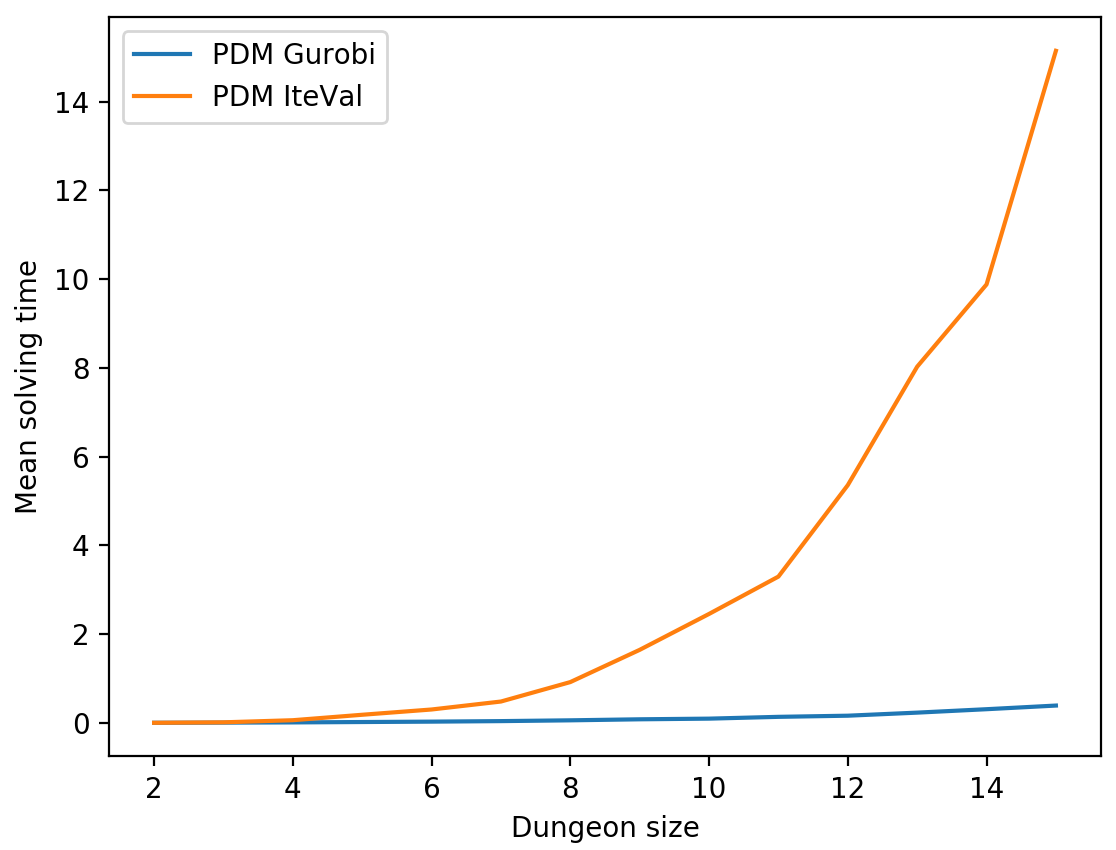
\includegraphics[width=\textwidth]{PlotSolvingTime.png}
		\caption{Temps moyen de résolution}
		\label{fig:solveTime}
	\end{subfigure}
	\begin{subfigure}[b]{0.48\textwidth}
		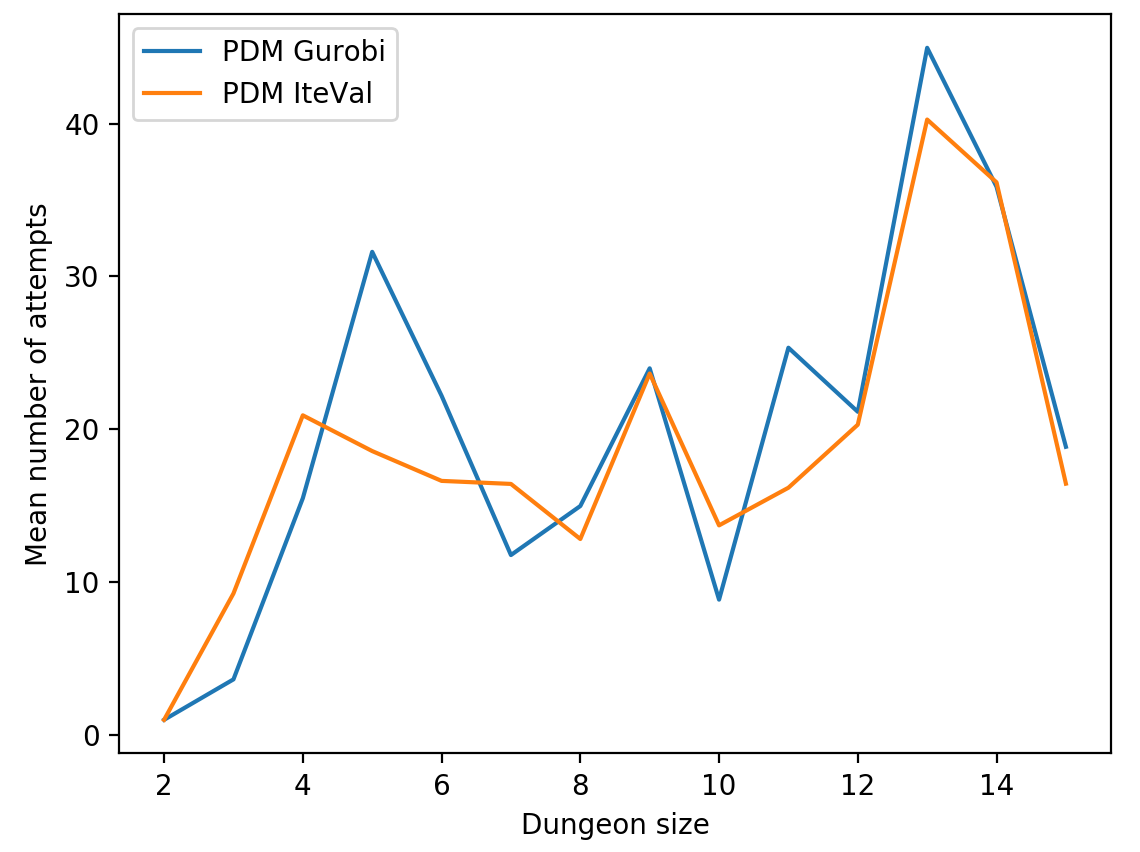
\includegraphics[width=\textwidth]{PlotNumAttemps.png}
		\caption{Nombre d'essai moyen avant la première victoire}
		\label{fig:numAttempts}
	\end{subfigure}
	\caption{Comparaison des résolution par itération de la valeur et par programmation linéaire}
	\label{fig:comparaisonAlgo}
\end{figure}


Nous avons aussi tracé le nombre d'essai moyen nécessaire pour obtenir une victoire, cela est présenté en Figure \ref{fig:numAttempts}. Cette figure ne permet cependant pas de dégager de tendance claire. Cela est sûrement dû au nombre de répétition (10) qui n'est pas suffisant pour avoir des moyennes pertinentes. De plus, nous faisons la moyenne sur des 10 instances de même taille mais très différente, la taille de l'instance n'est pas nécessairement corrélée à la probabilité de victoire.


Enfin, nous avons tracé le nombre moyen d'itération nécessaire à l'algorithme d'itération de la valeur pour atteindre sa solution optimal. Les résultats sont donnés en Figure \ref{fig:numIte}. La progression est relativement constante pour un nombre d'itération qui reste faible. Il faut cependant noter que le nombre d'itération est qu'un indicateur du temps de résolution. En effet le temps pour une itération est bien plus important pour les grands donjons que pour les plus petits.

\begin{figure}
	\centering
	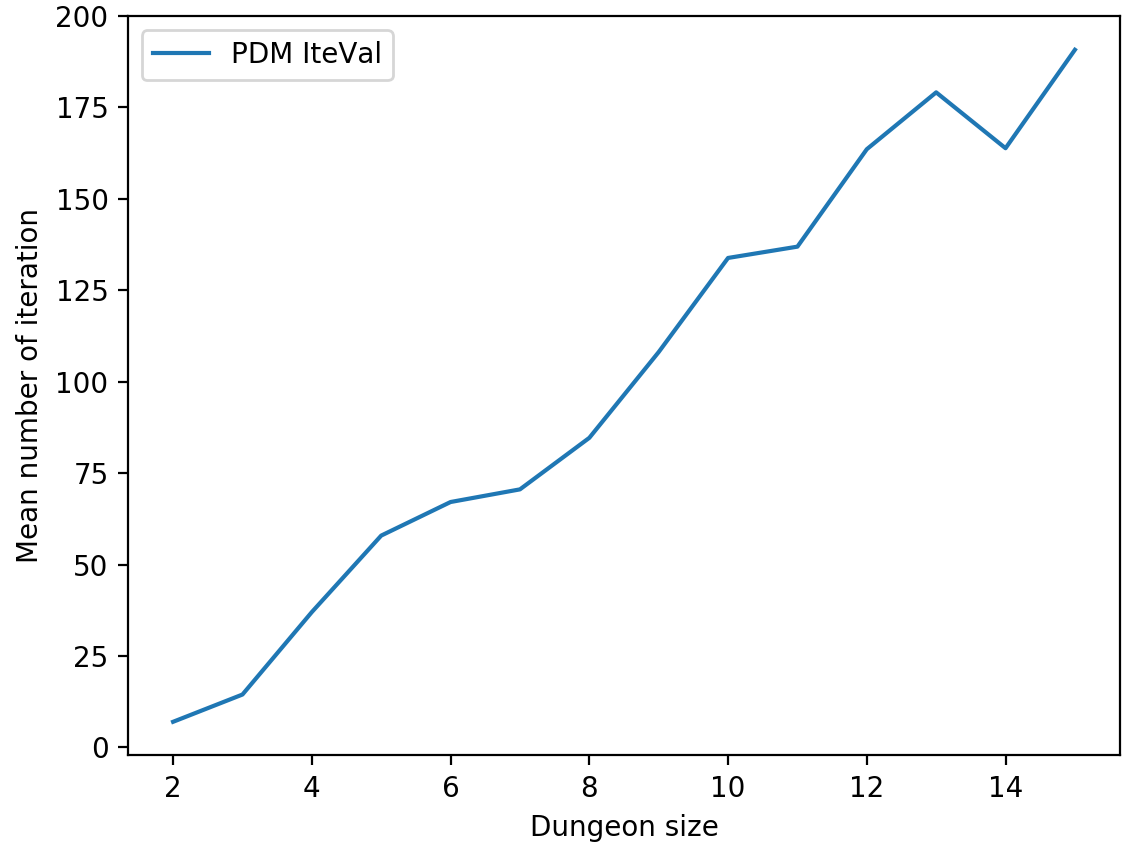
\includegraphics[scale=0.7]{PlotNumIte.png}
	\caption{Nombre de pas de l'algorithme d'itération de la valeur selon la taille du donjon}
	\label{fig:numIte}
\end{figure}

\section{Apprentissage par renforcement}

\end{document}